\documentclass[12pt]{article} 

\usepackage[utf8]{inputenc}    
\usepackage[T1]{fontenc}       
\usepackage{lmodern}           
\usepackage{amsmath, amssymb}  
\usepackage{graphicx}          
\usepackage{geometry}          
\usepackage{hyperref}          
\usepackage{fancyhdr}          
\usepackage{parskip}           
\usepackage{tikz}              
\usepackage{booktabs}          
\usepackage{enumitem}          
\usepackage{caption}           
\usepackage{listings}          
\usepackage{multirow}    
\usepackage{xcolor}      
\usetikzlibrary{automata, positioning}
\lstset{
  frame=tb,
  language=C,
  aboveskip=3mm,
  belowskip=3mm,
  showstringspaces=false,
  columns=flexible,
  basicstyle={\small\ttfamily},
  numbers=none,
  numberstyle=\tiny\color{gray},
  keywordstyle=\color{blue},
  commentstyle=\color{brown},
  stringstyle=\color{orange},
  breaklines=true,
  breakatwhitespace=true,
  tabsize=3
}
\hypersetup{
    colorlinks=true,
    linkcolor=blue,
    filecolor=magenta,      
    urlcolor=cyan,
    pdfpagemode=FullScreen,
    }

\geometry{margin=1in} 


\pagestyle{fancy}
\fancyhf{}
\fancyhead[L]{\leftmark} 
\fancyhead[R]{\thepage}  
\newtheorem{Correction}{Correction}

\title{CS3231 Tutorial 1}
\author{WANG Xiyu}
\date{\today}

\begin{document}

\maketitle

\tableofcontents 

\section{}
Show by induction that
\[
    1^2 + 2^2 + 3^2 + ... + n^2 = \frac{n(n+1)(2n+1)}{6}    
\]
\subsection*{Solution:}

To prove this by induction, 
\[
\sum_{i = 1}^{n} i^2 = \frac{n(n+1)(2n+1)}{6}
\]

\subsubsection*{Step 1: Base Case}
For \(n = 1\):
\[
\sum_{i=1}^{1} i^2 = 1^2 = 1
\]
\[
\frac{1(1+1)(2(1)+1)}{6} = \frac{1 \times 2 \times 3}{6} = 1
\]
The base case holds.

\subsubsection*{Step 2: Inductive Hypothesis}
Suppose that it holds for some \(n = k\):
\[
\sum_{i = 1}^{k} i^2 = \frac{k(k+1)(2k+1)}{6}
\]

\subsubsection*{Step 3: Inductive Step}
We need to show the formula holds for \(n = k+1\):
\[
\sum_{i=1}^{k+1} i^2 = \sum_{i=1}^{k} i^2 + (k+1)^2
\]
Using the inductive hypothesis:
\[
\sum_{i=1}^{k+1} i^2 = \frac{k(k+1)(2k+1)}{6} + (k+1)^2
\]
Factor \(k+1\) from both terms:
\[
\sum_{i=1}^{k+1} i^2 = \frac{(k+1)}{6} \left[k(2k+1) + 6(k+1)\right]
\]
Simplify the expression inside the brackets:
\[
\sum_{i=1}^{k+1} i^2 = \frac{(k+1)(k+2)(2k+3)}{6}
\]

\subsubsection*{Step 4: Conclusion}
Since the formula holds for \(n = 1\) and assuming it holds for \(n = k\) implies it holds for \(n = k+1\), by the principle of mathematical induction, the formula
\[
\sum_{i = 1}^{n} i^2 = \frac{n(n+1)(2n+1)}{6}
\]
is true for all positive integers \(n\).

\section{}
For a particular alphabet set \(\Sigma\), how many strings of length n are there in \(\Sigma^*\)? 
How many strings in \(\Sigma^*\) have length \(\leq\) n?

\subsection*{2.1: \(|s| = n\)}
It is obvious that 
\[
\forall n \in \mathbb{N}, \forall s \in \Sigma^*, (|s| = n) \implies \forall i \in \{1, 2, \dots, n\}, \exists \sigma \in \Sigma \text{ such that } s_i = \sigma
\]
The number of choices per postion is 
\[|\Sigma|\]
The number of strings of length \( n \) is given by:
\[
\text{Number of strings of length } k = |\Sigma| \times |\Sigma| \times \cdots \times |\Sigma| = |\Sigma|^n
\]

\subsection*{2.2: \(|s| \leq n\)}
From \((2.1)\), 
\[
\text{Number of strings of length } k = |\Sigma| \times |\Sigma| \times \cdots \times |\Sigma| = |\Sigma|^n
\]

\[
\text{Number of strings of length} \leq k = |\Sigma|^0 \times |\Sigma|^1 \times \cdots \times |\Sigma|^n = \sum_{i=0}^{n}|\Sigma|^i
\]
Simplifying this geometric series gives:
\[\sum_{i=0}^{n}|\Sigma|^i = \frac{|\Sigma|^{n+1}-1}{|\Sigma|-1}\]
\begin{Correction}
    \textcolor{red}{Geometric series doesnt work on \(|\Sigma| = 1\)}
\end{Correction}
\section{}
\subsection*{Prove:}
\[
A\cdot\bigcup\limits_{i=1}^{\infty} B_i=\bigcup\limits_{i=1}^{\infty}A\cdot B_i
\]
\subsubsection*{Solution:}
Suppose:
\[s\in A\cdot\bigcup\limits_{i=1}^{\infty} B_i\]
By the definition of concatenation,
\[s = a \cdot b \implies \exists a, b (a \in A, b\in\bigcup\limits_{i=1}^{\infty} B_i )\]
\[b\in\bigcup\limits_{i=1}^{\infty} B_i \implies\exists j \in \mathbb{N}(b \in B_j)\]
\[s = a \cdot b \implies s \in \bigcup\limits_{j=1}^{\infty}A\cdot B_j\]
Thus,
\[
A\cdot\bigcup\limits_{i=1}^{\infty} B_i \subseteq \bigcup\limits_{i=1}^{\infty}A\cdot B_i   \text{      (1)}
\]

Suppose:
\[s\in \bigcup\limits_{i=1}^{\infty}A\cdot B_i\]
By the definition of union,
\[s = a \cdot b\]
\[\exists j \in \mathbb{N}(s \in A\cdot B_j)\]
By the definition of concatenation,
\[s = a \cdot b \implies \exists a, b (a \in A, b\in B_j )\]
\[b\in B_j \land B_j \in \bigcup\limits_{i=1}^{\infty}B_i \implies b \in \bigcup\limits_{i=1}^{\infty}B_i\]
Therefore, 
\[s = a\cdot b \in A \cdot \bigcup\limits_{i=1}^{\infty}B_i\]
Thus,
\[
 \bigcup\limits_{i=1}^{\infty}A\cdot B_i\subseteq A\cdot\bigcup\limits_{i=1}^{\infty} B_i \text{      (2)}
\]
From \((1)\) and \((2)\),
\[
A\cdot\bigcup\limits_{i=1}^{\infty} B_i=\bigcup\limits_{i=1}^{\infty}A\cdot B_i
\]

\begin{itemize}
    \item \textcolor{red}{Note: properties hold on finite union cannot be assumed on infinite union.}
\end{itemize}

\subsection*{Prove:} 
\[
(A^*)^+=(A^+)^*
\]
\subsubsection*{Solution:}
\[(A^*)^+ = A^* \cup (A^*)^2 \cup (A^*)^3 \cup ... \]
\[= (\{\epsilon\} \cup A \cup A^2 \cup A^3 \cup ...) \cup (\{\epsilon\} \cup A \cup A^2 \cup A^3 \cup ...) \cup ...\]
\[= \{\epsilon\} \cup A \cup A^2 \cup A^3 \cup ...  \text{   (LHS)}\] 

\[(A^+)^* = \{\epsilon\} \cup A^+ \cup (A^+)^2 \cup ...\]
\[= \{\epsilon\} \cup (A \cup A^2 \cup A^3 \cup ...)\cup (A \cup A^2 \cup A^3 \cup ...)\cup ...\]
\[= \{\epsilon\} \cup A \cup A^2 \cup A^3 \cup ...  \text{   (RHS)}\] 

To prove 

\begin{Correction}
    \textcolor{red}{\newline
        To Prove \(A^* \subseteq (A^*)^*\) \newline
        Let \(B = (A)^*\)
        \(A \subseteq (B)^*\)   \newline
        To Prove \((A^*)^* \subseteq A^*\)\newline
        Suppose \(\)
    }
\end{Correction}


\section{}
I'm too lazy to do this drawing here please refer to the photo attached below.
\begin{figure}[htbp]
    \centering
    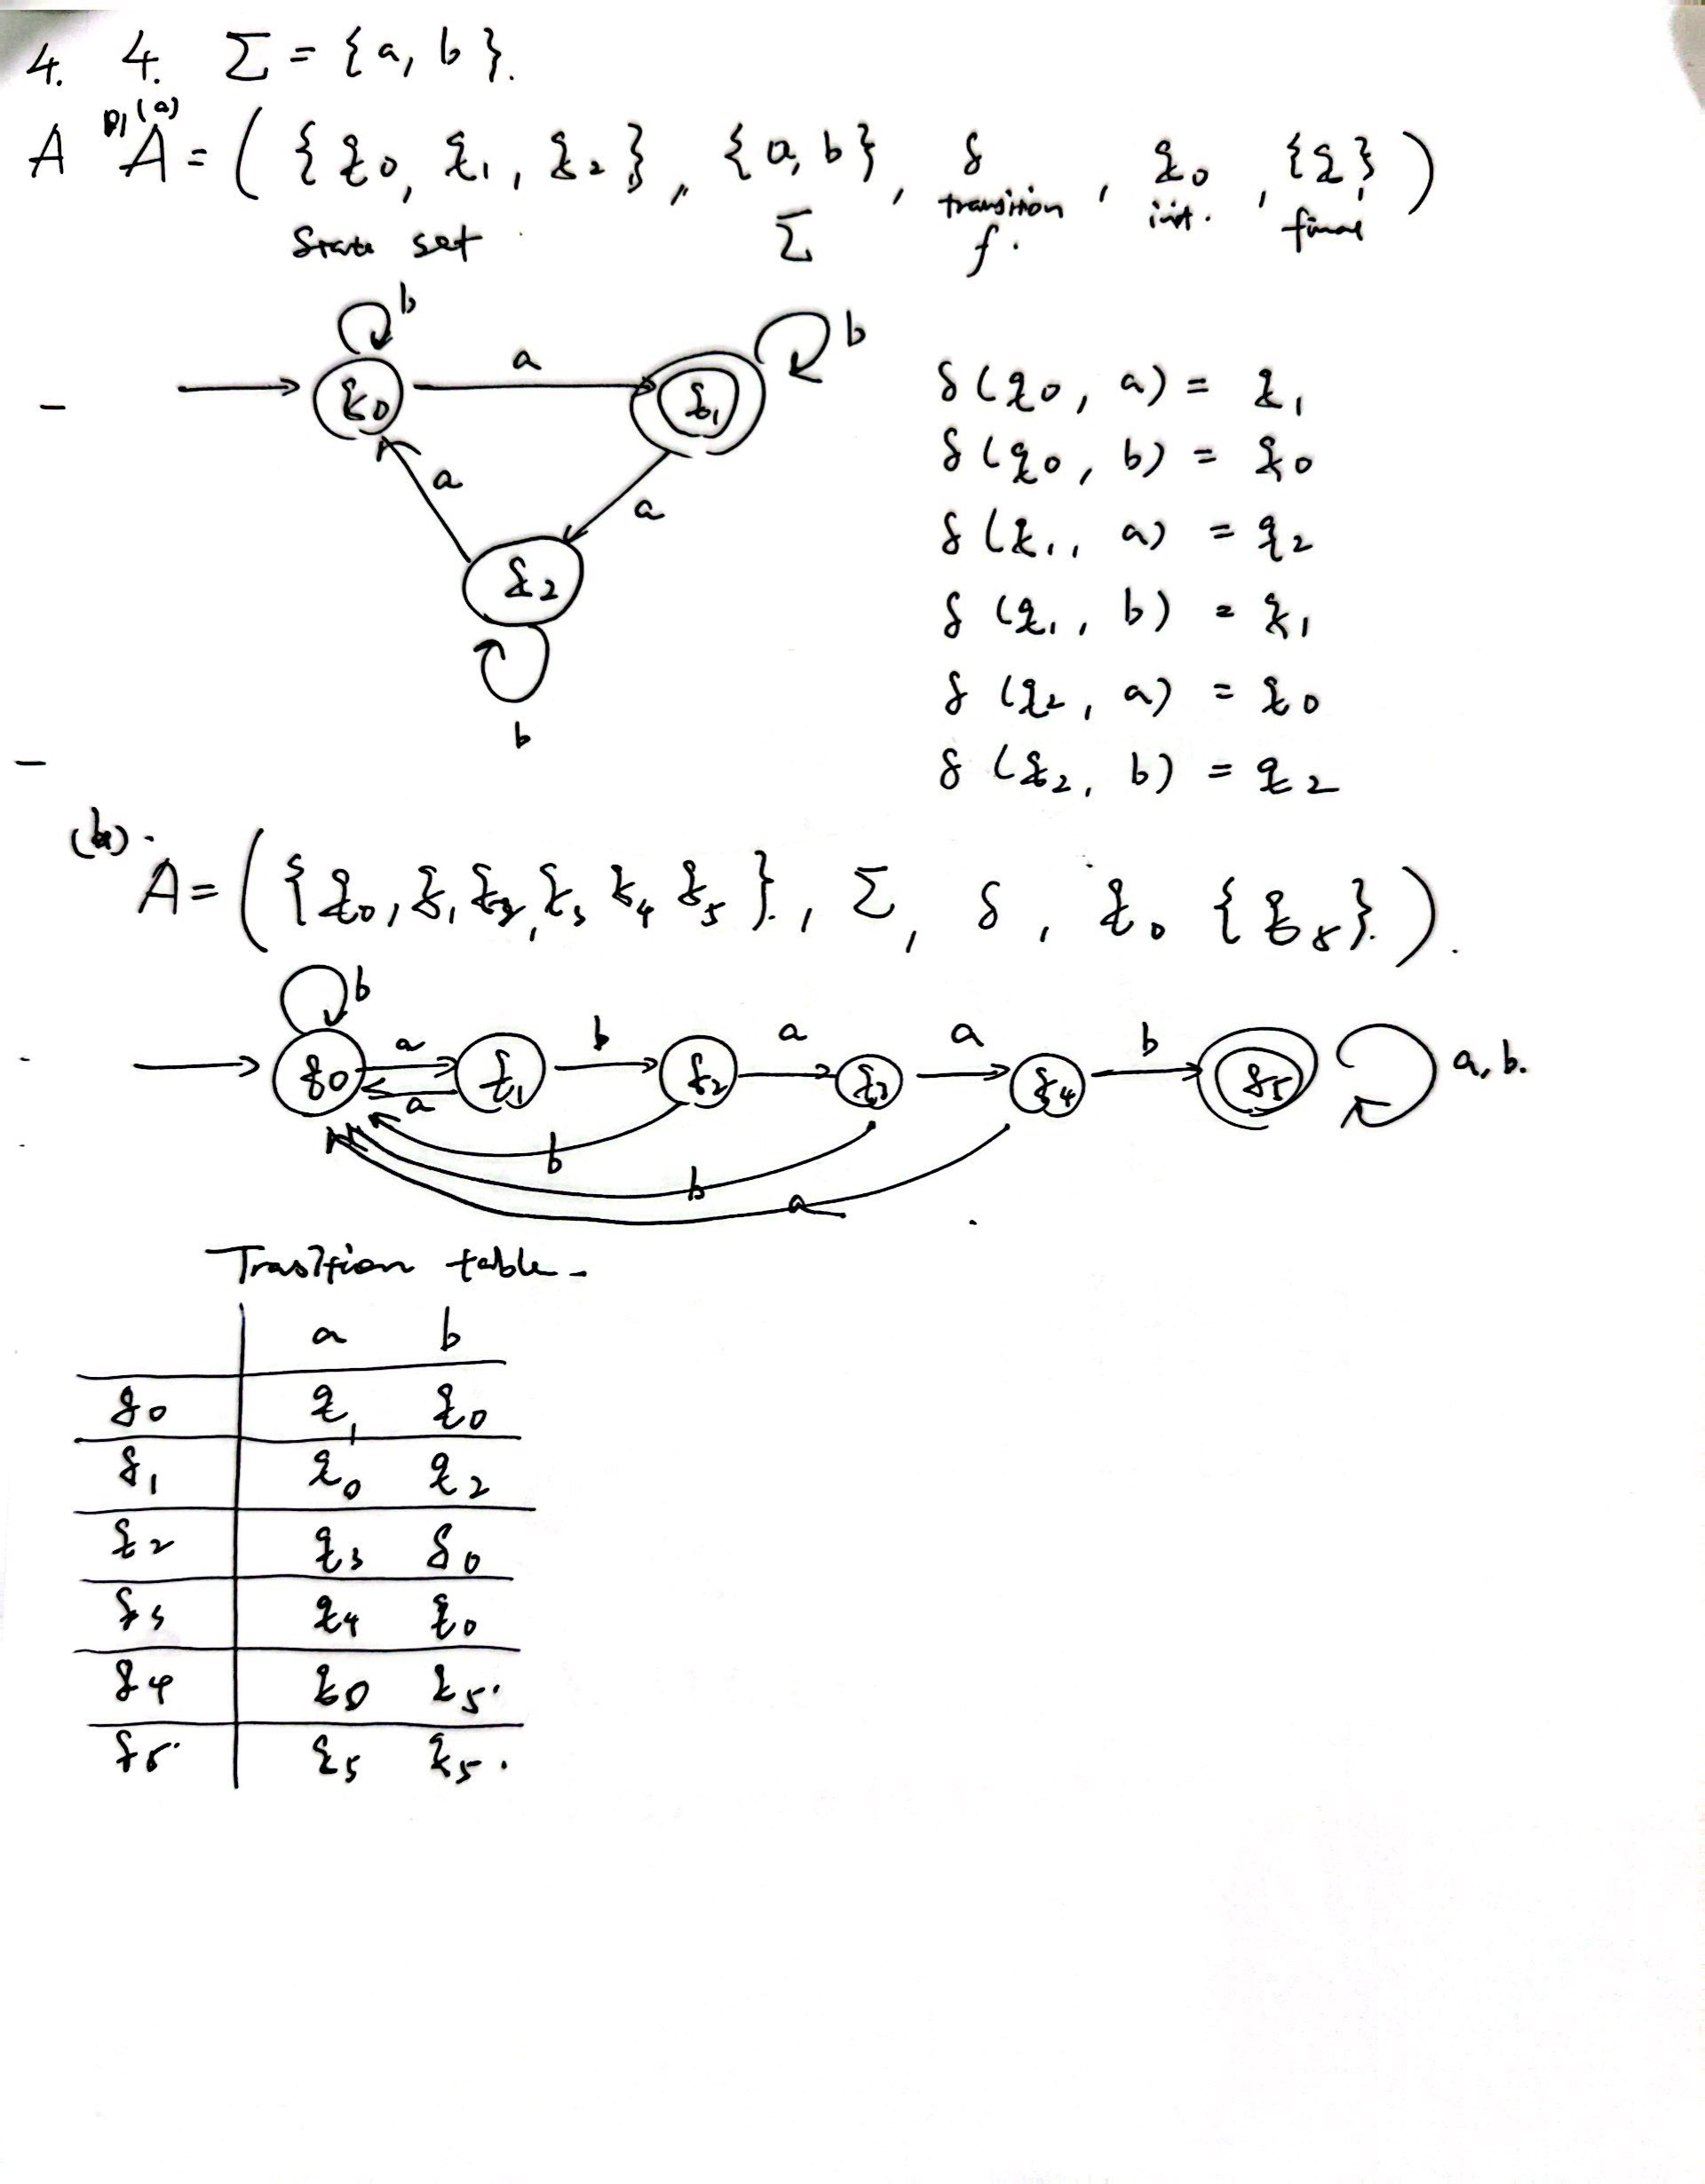
\includegraphics[width=\textwidth]{Tut1/4ab.jpg}
    \caption{Full-size image example}
    \label{fig:fullsize}
\end{figure}
\begin{figure}[htbp]
    \centering
    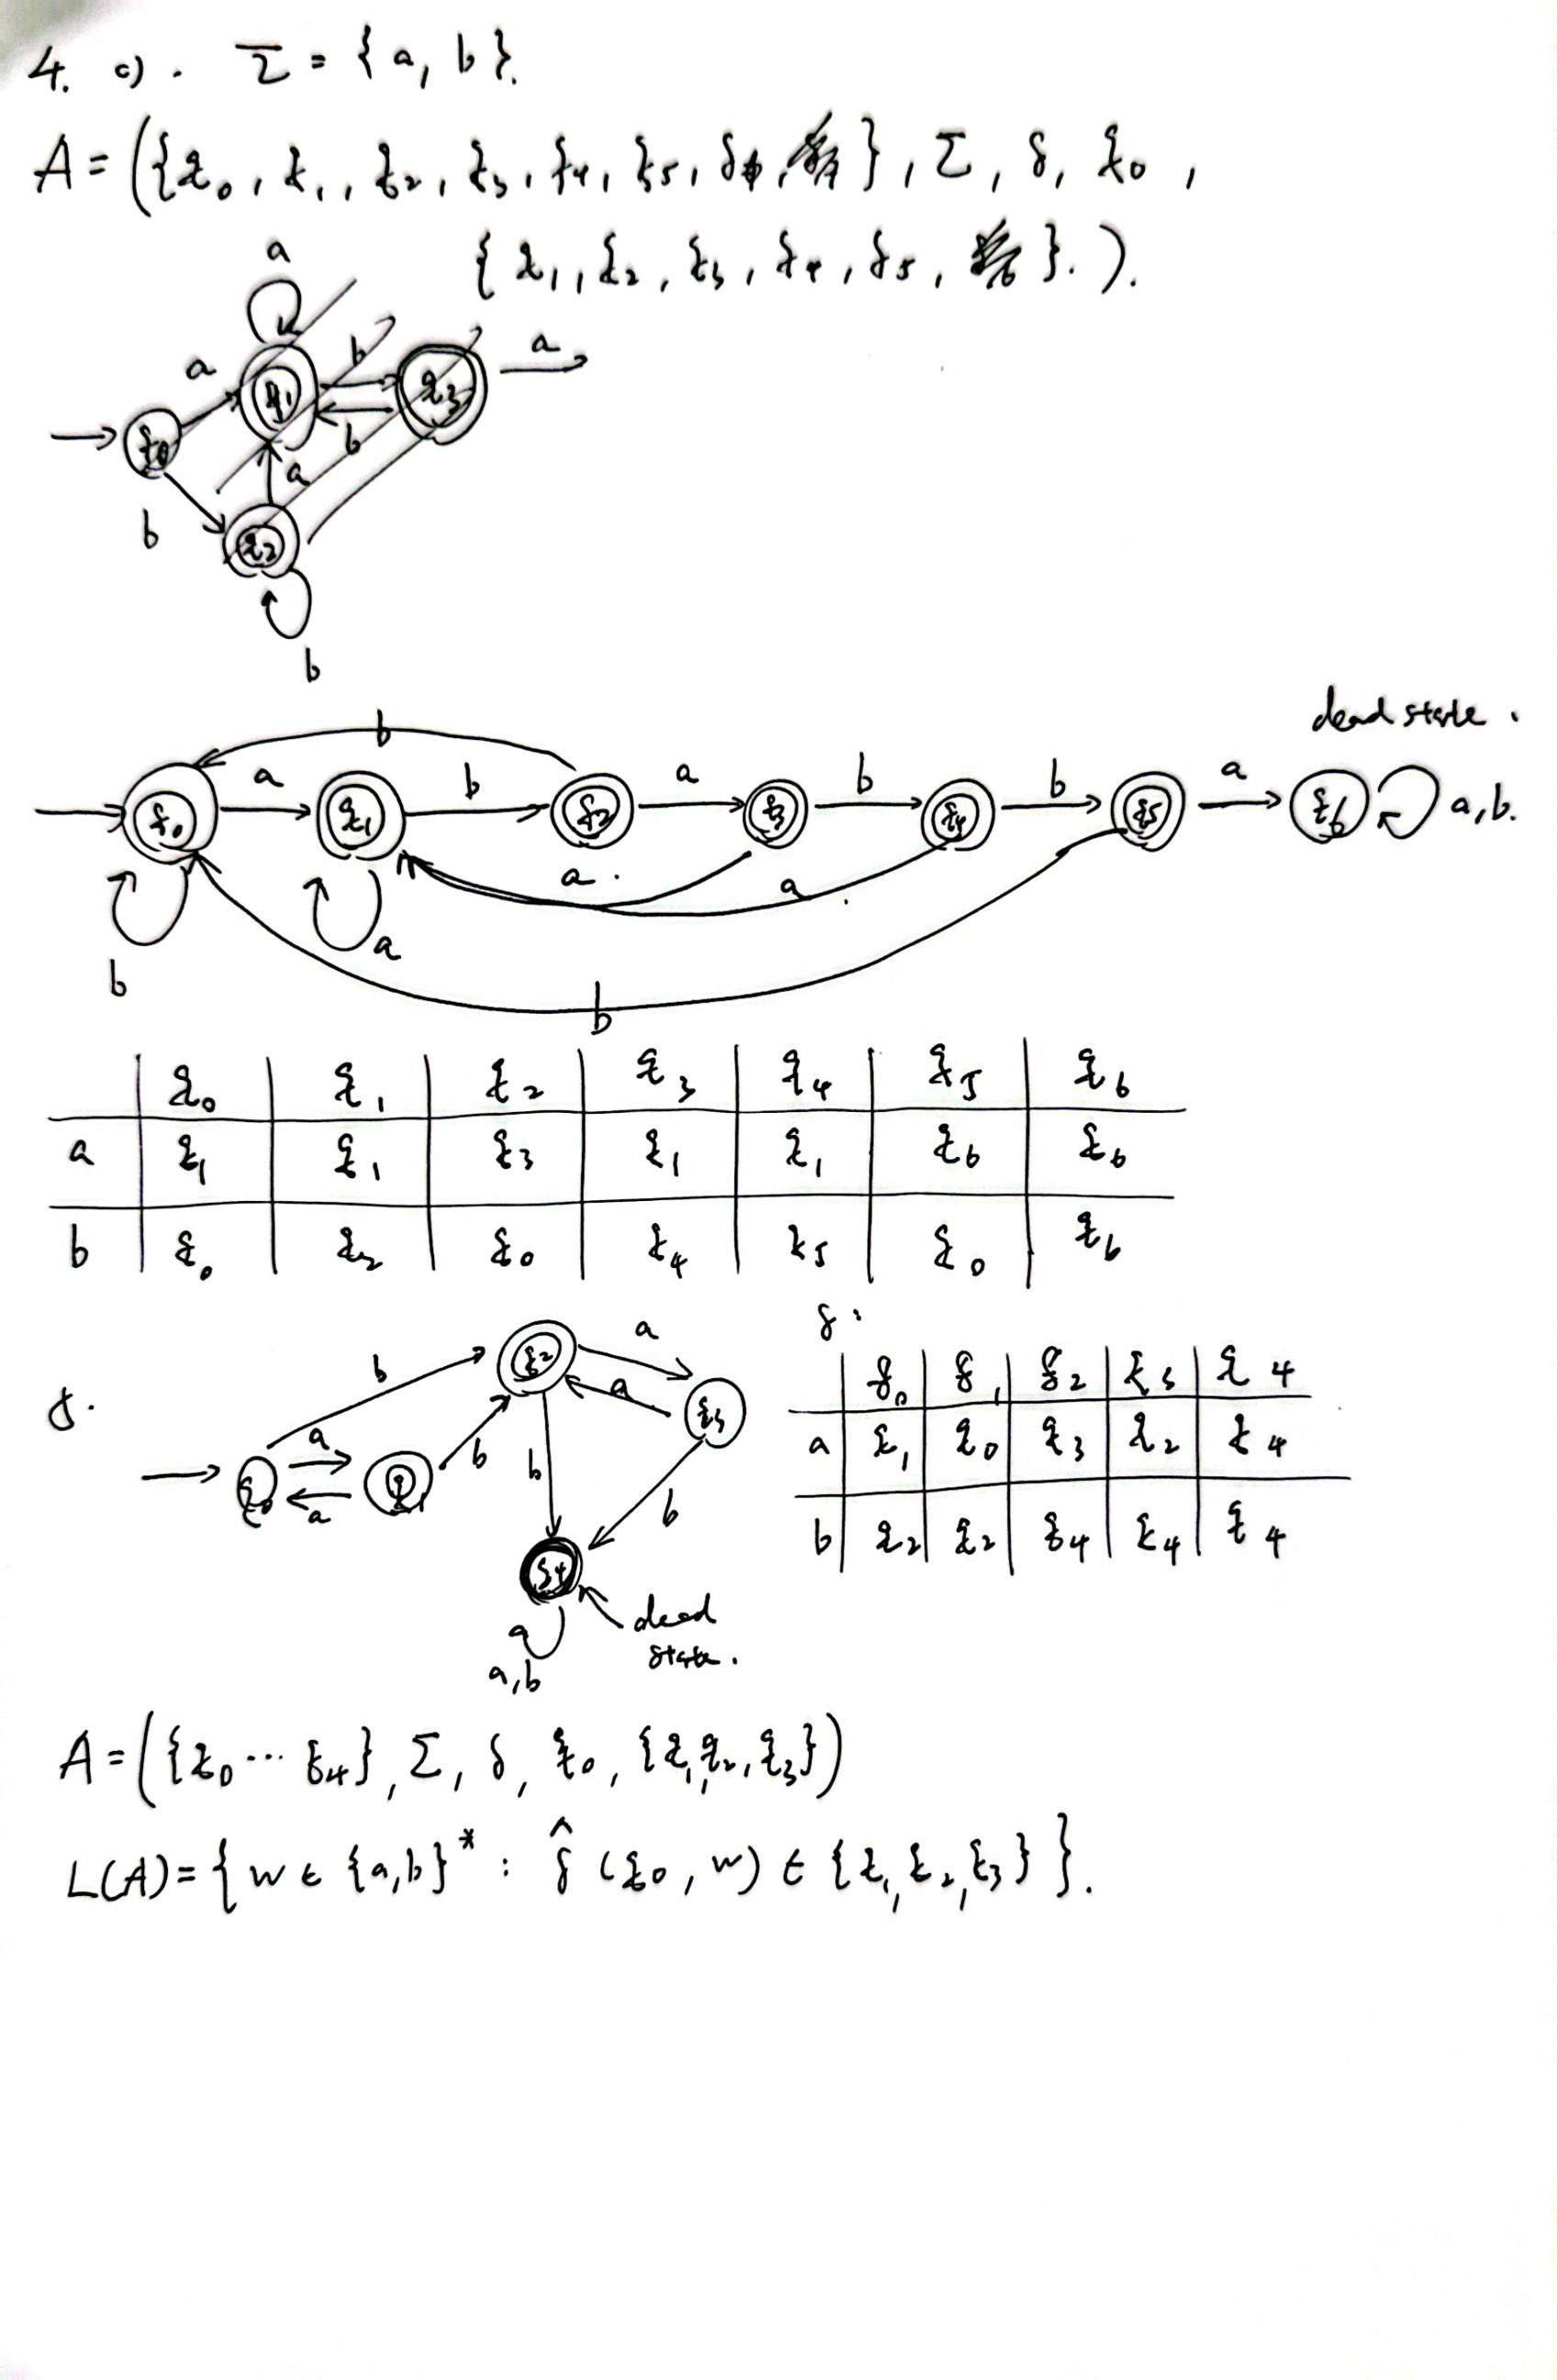
\includegraphics[width=\textwidth]{Tut1/4c.jpg}
    \caption{Full-size image example}
    \label{fig:fullsize}
\end{figure}
\newpage
\section{}
\begin{center}
    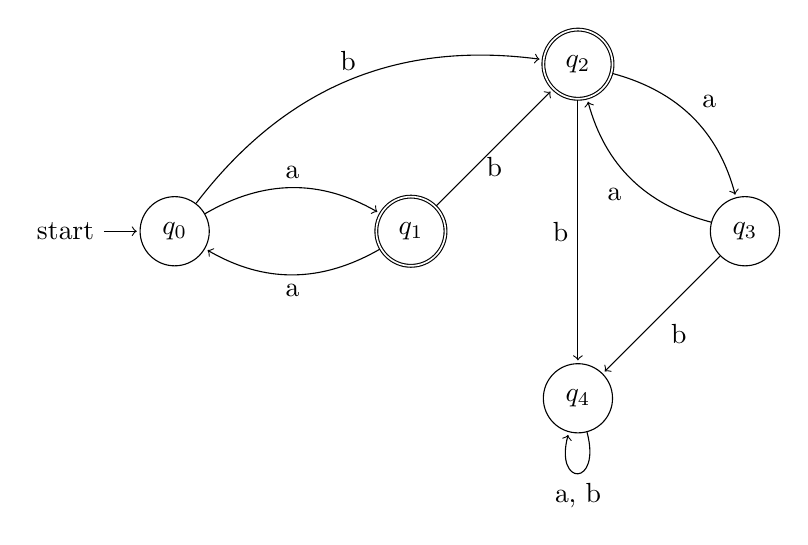
\begin{tikzpicture}[shorten >=1pt, node distance=3cm, on grid, auto]
        
        \node[state, initial] (q_0) {$q_0$}; 
        \node[state, accepting] (q_1) [right=of q_0] {$q_1$}; 
        \node[state, accepting] (q_2) [above right=of q_1] {$q_2$}; 
        \node[state] (q_3) [below right=of q_2] {$q_3$};
        \node[state] (q_4) [below right=of q_1] {$q_4$};
        
        \path[->] 
        (q_0) edge[bend left, above] node {a} (q_1)
        (q_0) edge[bend left, above] node {b} (q_2)
        (q_1) edge[bend left, below] node {a} (q_0)
        (q_1) edge[below] node {b} (q_2)
        (q_2) edge[bend left, above right] node {a} (q_3)
        (q_2) edge[left] node {b} (q_4)
        (q_3) edge[bend left, below left] node {a} (q_2)
        (q_3) edge[below right] node {b} (q_4)
        (q_4) edge[loop below] node {a, b} ();
    \end{tikzpicture}
\end{center}
This DFA contains 2 accepting states, suggesting the union of the language accepted at state 1 and state 2.
\begin{itemize}
    \item The language accepted at state 1 is 
    \begin{itemize}
        \item Case 1-1: \(a(aa)^*\).
    \end{itemize}
    \item The language accepted at state 2 can be 
    \begin{itemize}
        \item  Case 2-1: \((aa)^*b\): ((0 - 1 - 0)\(^*\) - 2) (\(Case\ 2-1 \subseteq Case\ 2-3\))
        \item  Case 2-2: \((aa)^*b(aa)^*\):  ((0 - 1 - 0)\(^*\) - (2 - 3 - 2)\(^*\)) (\(Case\ 2-2 \subseteq Case\ 2-4\))
        \item  Case 2-3: \(a^*(aa)^*b\):  (0 - (1 - 0 - 1)\(^*\) - 2) (\(Case\ 2-3 \subseteq Case\ 2-2\))
        \item  Case 2-4: \(a^*(aa)^*b(aa)^*\):  (0 - (1 - 0 - 1)\(^*\) - (2 - 3 - 2)\(^*\))
        \item  Case 2-5: \(b(aa)^*\): (0 - (2 - 3 - 2)\(^*\)) (\(Case\ 2-5 \subseteq Case\ 2-2\))
    \end{itemize}
\end{itemize}
All unioned together, language accepted by this DFA is 
    \begin{center}
        \[L = a(aa)^* \cup a^*(aa)^*b(aa)^*\]
    \end{center}
    \begin{Correction}
        \textcolor{red}{\[L = a(aa)^* \cup a^*b(aa)^*\]
        Since \(a^*(aa)^*\) accommendate both even and odd number of a's}

    \end{Correction}
x
\section{}
\begin{center}
    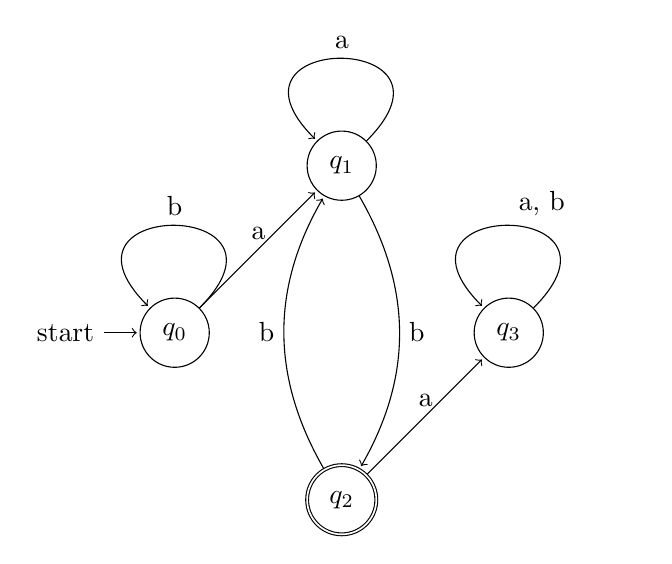
\begin{tikzpicture}[shorten >=1pt, node distance=3cm, on grid, auto]
        \node[state, initial] (q_0) {$q_0$}; 
        \node[state] (q_1) [above right=of q_0] {$q_1$}; 
        \node[state, accepting] (q_2) [below right=of q_0] {$q_2$}; 
        \node[state] (q_3) [below right=of q_1] {$q_3$};
        \path[->] 
        (q_0) edge[loop, above] node {b} ()
        (q_0) edge[above] node {a} (q_1)
        (q_1) edge[loop, above] node {a} ()
        (q_1) edge[bend left, right] node {b} (q_2)
        (q_2) edge[bend left, left] node {b} (q_1)
        (q_2) edge[above] node {a} (q_3)
        (q_3) edge[loop, above right] node {a, b} ();
    \end{tikzpicture}
\end{center}
\begin{itemize}
    \item The language accepted at state 2 is 
    \begin{itemize}
        \item Case 1: Looping on \(q_0\), looping on \(q_1\), enter \(q_2\):
            \[L_1 = b^*(a)(a)^*b\]
        \item Case 2: From \(q_2\), looping on \(q_1\) and eventually go back to \(q_2\):
            \[L_2 = b^*(a)(a)^*b(b(a)^*b)^*\]
    \end{itemize}
    
\end{itemize}
Unioned together, 
    \begin{center}
        \[L = L_1 \cup L_2 = b^*aa^*b(ba^*b)^*\]
    \end{center}

 
\end{document}
